\begin{frame}
\frametitle{Properties of fibres (St. Gobain)}
\begin{columns}
\column{0.35\textwidth}
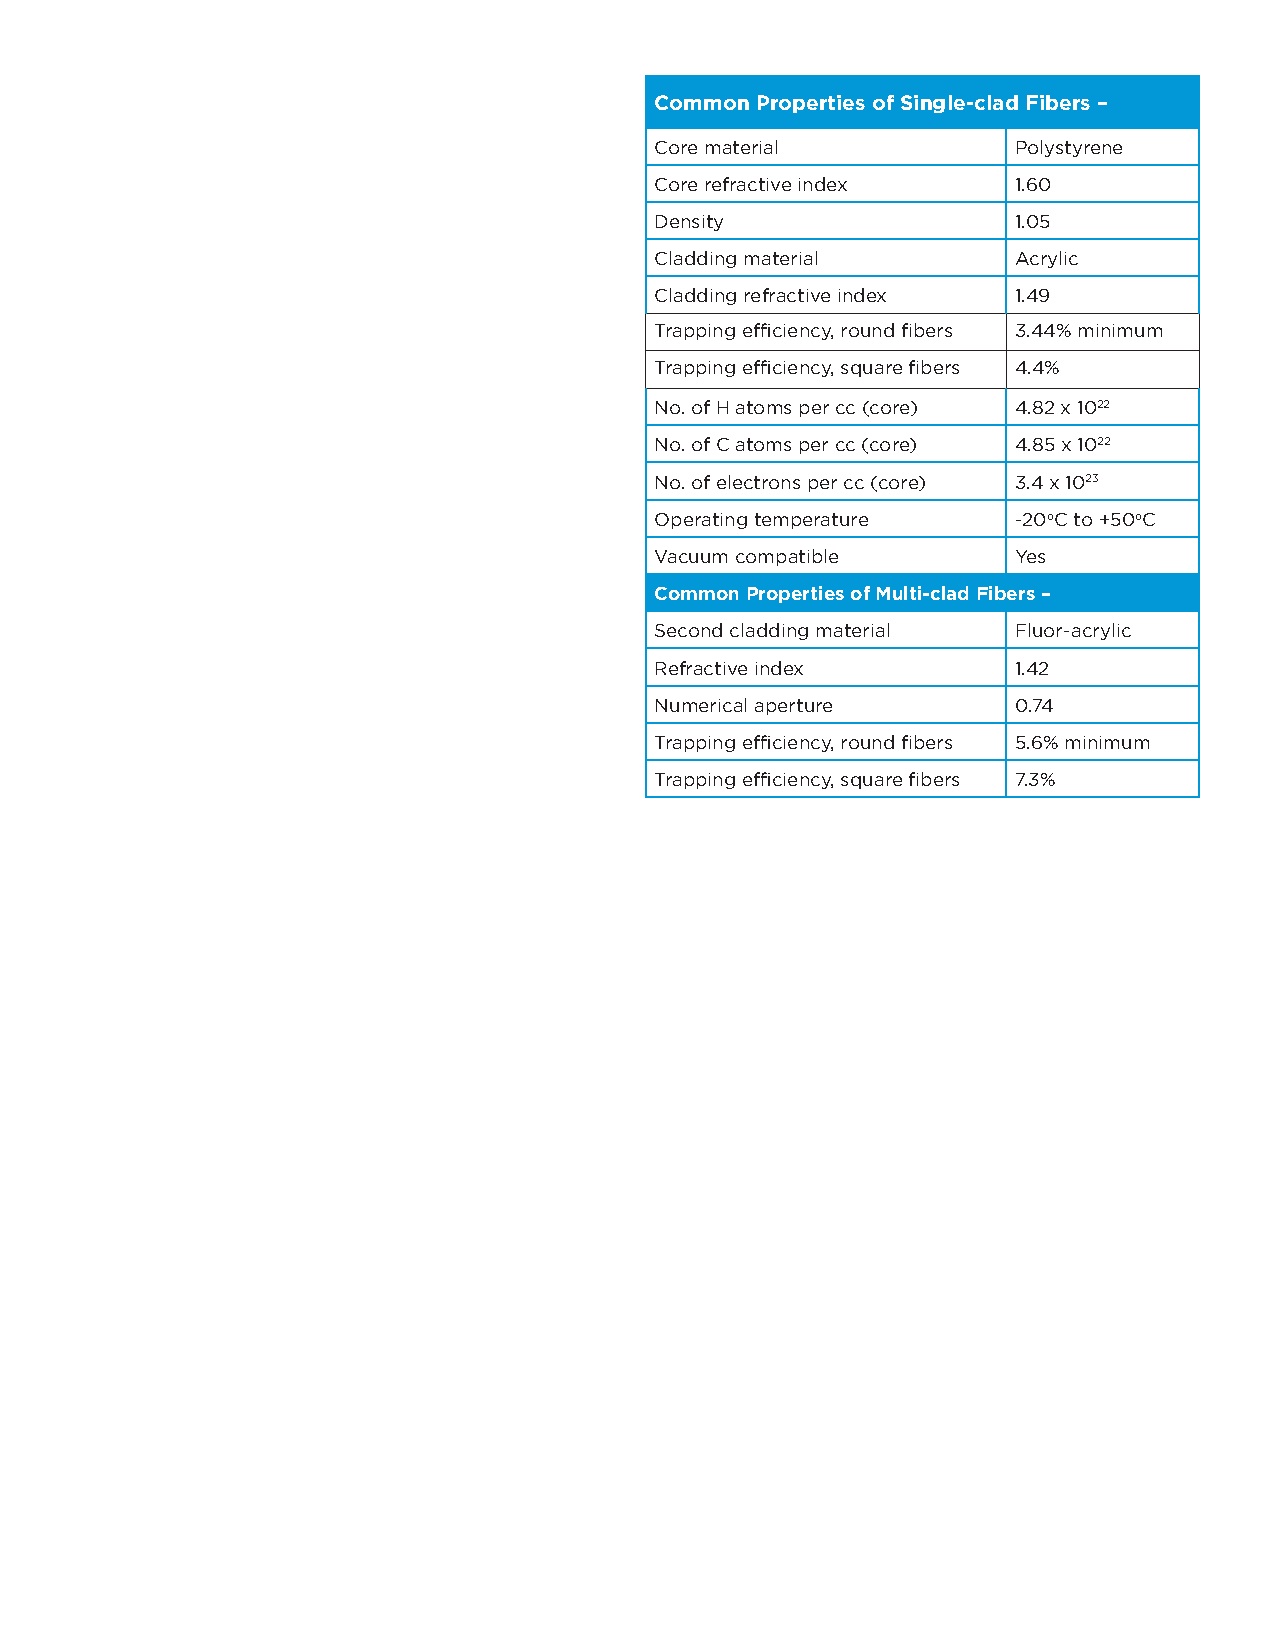
\includegraphics[scale=0.5]{img/fibersStGobain.pdf}
$\bullet$ Att. length for SG WLS fibres $>3.5$m.
  
 \column{0.5\textwidth}
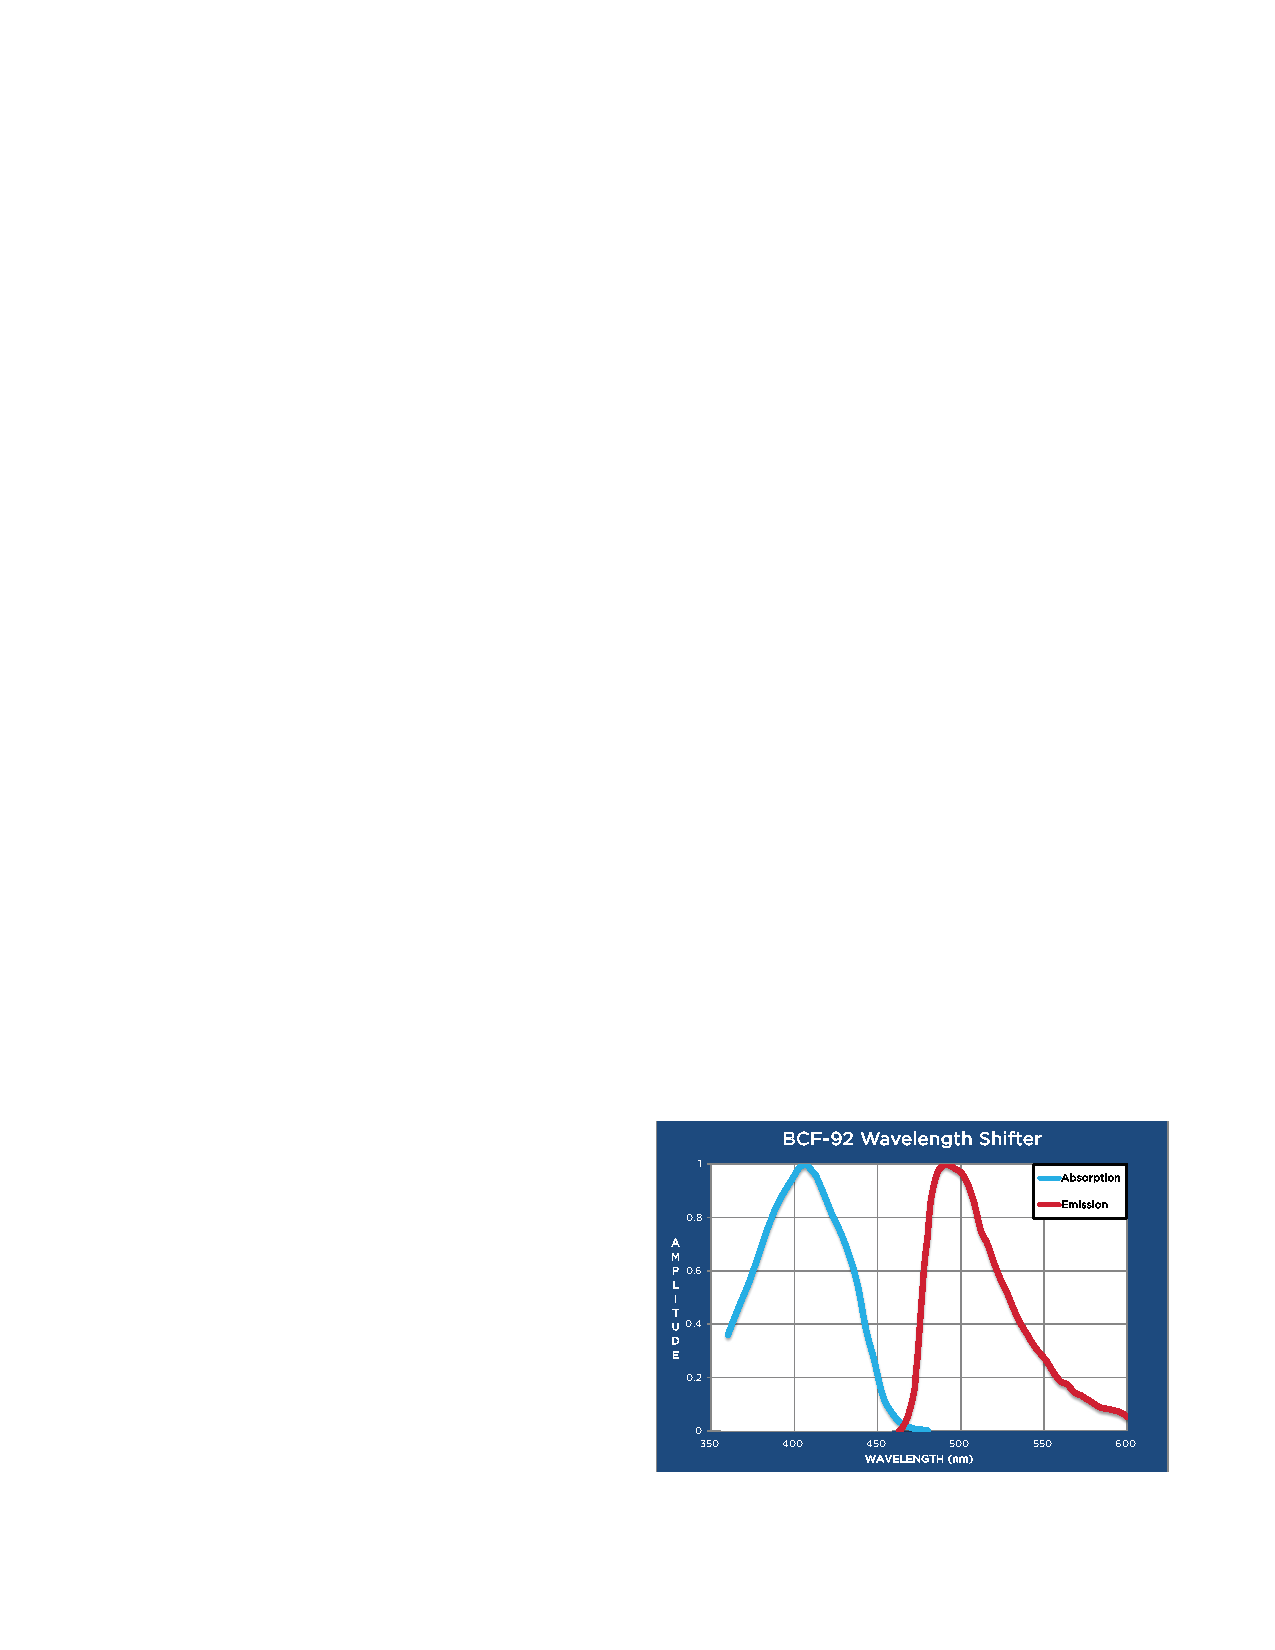
\includegraphics[scale=0.5]{img/wlsStGobain.pdf}

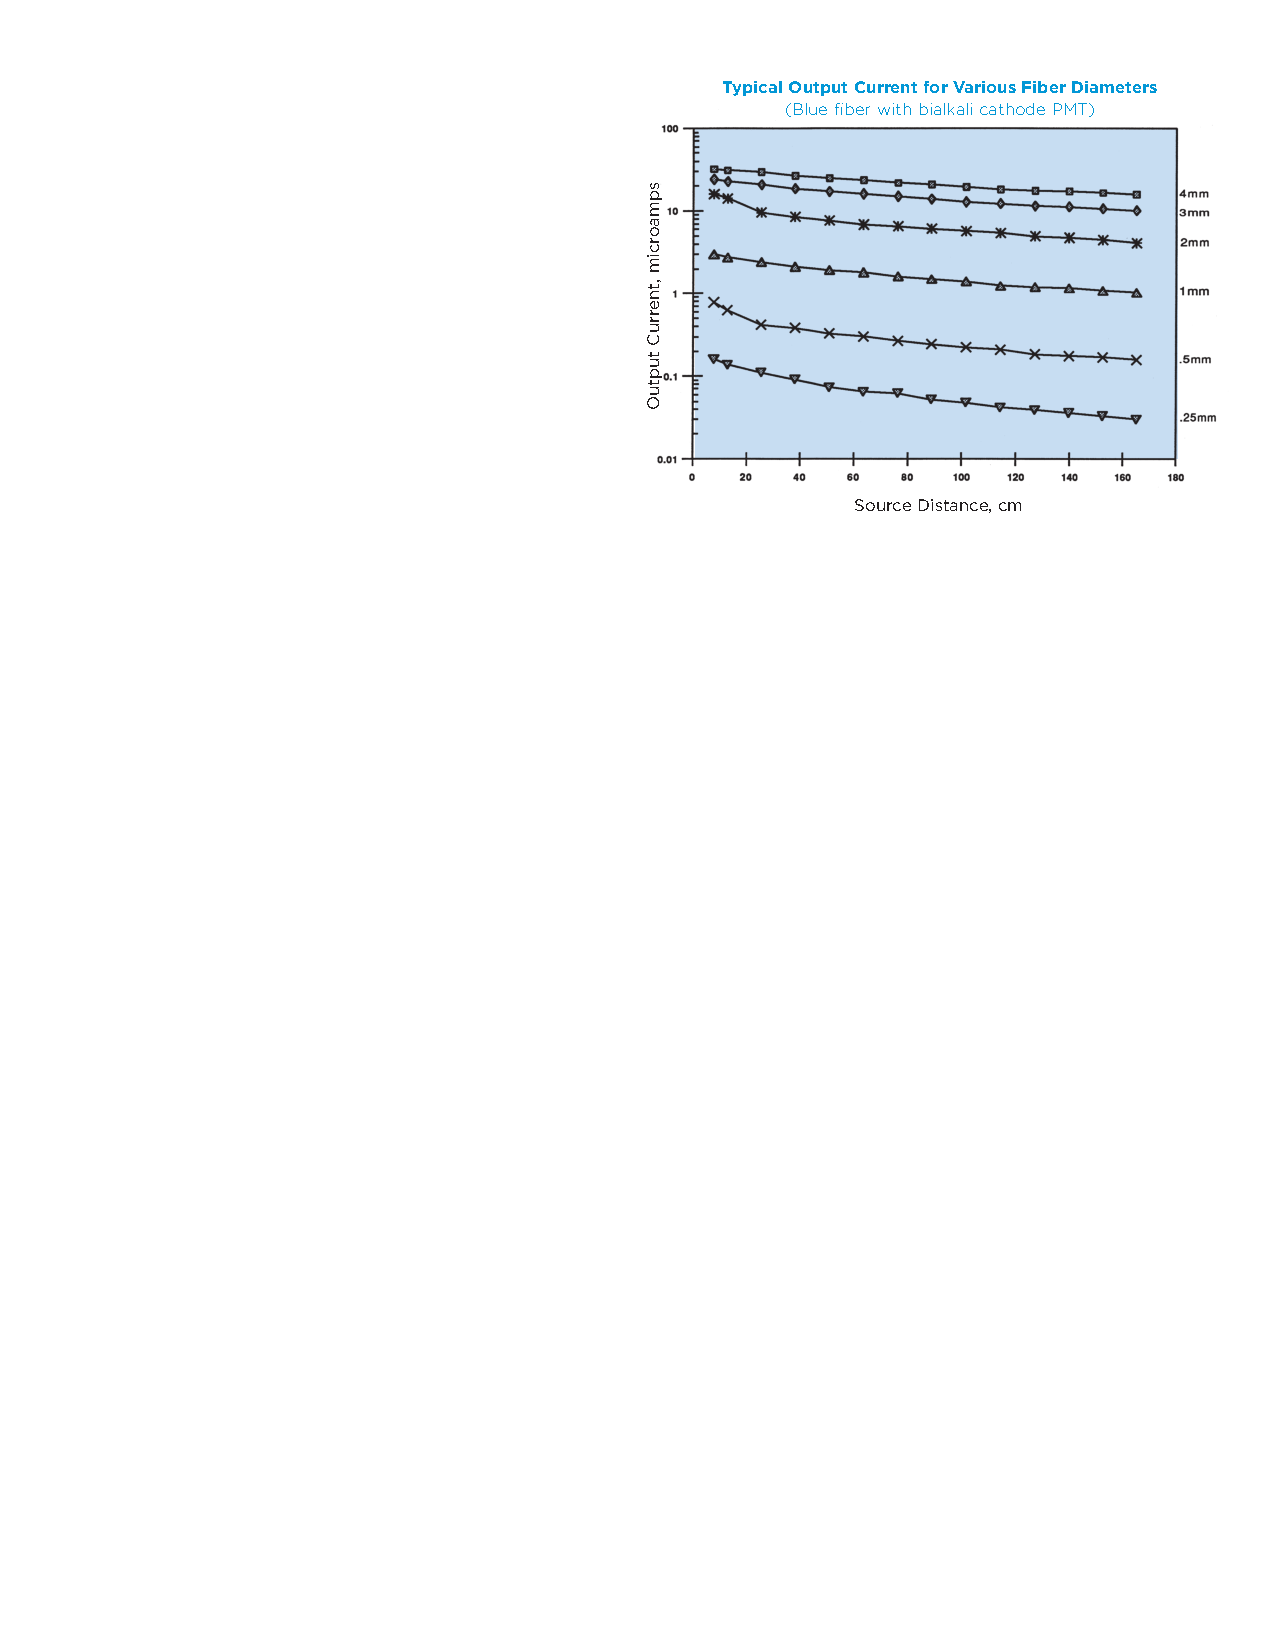
\includegraphics[scale=0.5]{img/fibAttLength.pdf}

\end{columns}
\end{frame}

\begin{frame}
\frametitle{Measuring \sone\ with fibers}


$\bullet$ The overall light collection efficiency of the BFD has been computed using full Monte Carlo simulation (JVM). A value of 3.0 \% is obtained assuming a QE  for TPB of 0.65 and squared fibres of \SI{2}{mm} size. Using previous values of QE for TPB (75\%) we find up to 3.5 \%. Finding a primary WLS with a QE $\sim$ 85\% would yield an efficiency of 4\%. 

$\bullet$ Adding one AFD will add an extra efficiency of 1.5 \% (QE $=$0.65) to
 2.0 \% (QE $=$0.85). Thus the combined efficiency of the BFD and AFD vary from
 4.5\% to 6\%. We will take 5\% as default value. 
\end{frame}

\begin{frame}
\frametitle{Reading fibres with SiPMs}
\begin{columns}
\column{0.45\textwidth}

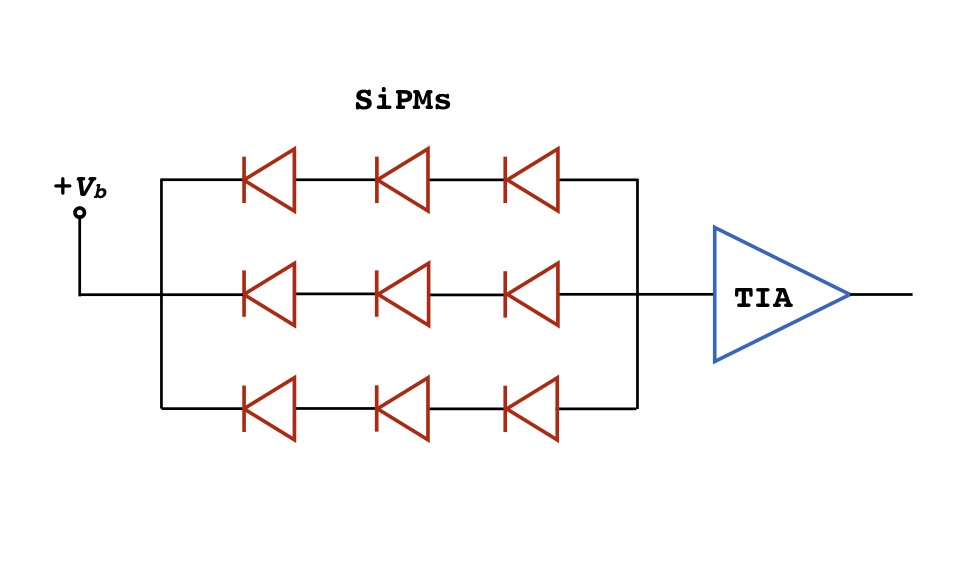
\includegraphics[scale=0.5]{img/3s3p.png}

$\bullet$ Each fibre can be read out with 4 SiPMs of \SI{1 x 1}{mm^2}, connected in a 2s2p scheme, similar to the 3s3p scheme used by Dark Side. This means that two pairs of SiPMs are connected in parallel and then the pairs connected in series. The overall effect is that the amplitude and capacitance of the system is the same than 1 SiPM of \SI{1 x 1}{mm^2}.
  
\column{0.45\textwidth}
 
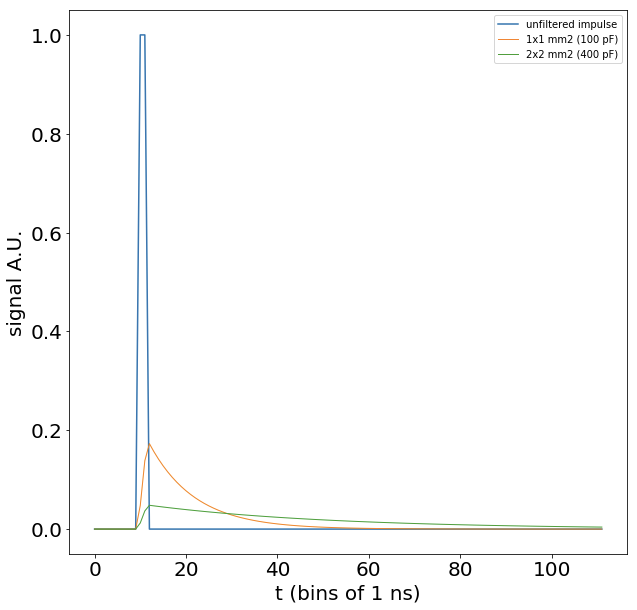
\includegraphics[scale=0.2]{img/sipmResponse2s2p.png}

$\bullet$ Given the relatively small capacitance of the 2s2p arrangement, the baseline is restored in \SI{50}{ns}. Sampling at 20 MHz is then possible to measure \sone\ in \SI{50}{ns}, integrating only the DCR corresponding to that interval. 

\end{columns}
\end{frame}

\begin{frame}
\frametitle{Signal and DCR for \sone}
\begin{columns}
\column{0.35\textwidth}


{\fontsize{6pt}{7.2}\selectfont 
\begin{table}
\begin{center}
\begin{tabular}{|l|l|}
\hline
\# fibers (2.0 mm) & \num{3.93e+03} \\
\# electronic channels  & \num{7.85e+03} \\
\#  SiPMs (\SI{1 x 1}{mm^2}) &  \num{3.14e+04} \\
Sc. phot. det. (Kr) &  \num{2.14e+01}\\
Sc. phot. det. (Qbb) &\num{1.27e+03} \\
Sc. phot. det.  per Fiber (Kr) & \num{5.45e-03} \\
Sc. phot. det. per Fiber (Qbb) & \num{3.23e-01} \\
 \hline
\end{tabular}
\end{center}
\end{table}%
}
\column{0.45\textwidth}
 
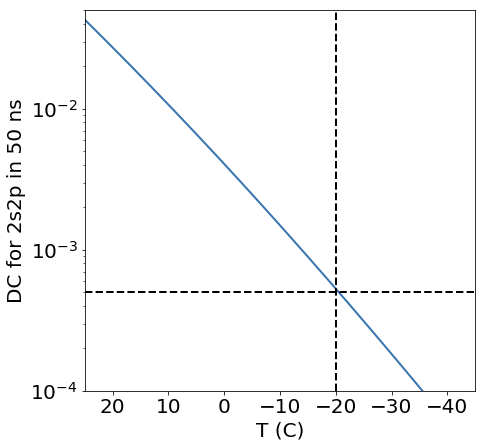
\includegraphics[scale=0.3]{img/dcrFibers2s2p.png}

\end{columns}
\blt {\bf Operating at \SI{-20}{\celsius} is possible to reduce DCR one order of magnitude below \sone\ signal at Kr (much better than that at \Qbb. Operation in the range \SIrange{-10}{-20}{\celsius} appears possible}. 
\end{frame}

\begin{frame}
\frametitle{Measuring \stwo}

\begin{table}
\begin{center}
\begin{tabular}{|l|l|}
\hline
EL phot. det. (Kr) &  \num{1.82e+04}\\
EL phot. det. (Qbb) &\num{1.08e+06} \\
EL phot. det.  per Fiber (Kr) & \num{4.63e+00} \\
EL phot. det. per Fiber (Qbb) & \num{2.74e+02} \\
 \hline
\end{tabular}
\end{center}
\end{table}

\blt\ No problems o dynamic range. Sampling at $\sim$\SI{2}{\micro\second} appears
straight forward. Photoelectron statistics is very large and does not affect the energy resolution. 
\end{frame}
